\chapter{Orthogonal Projective Double Covers}
\label{4classbip}
Throughout this thesis we have examined many different spherical $t$-distance sets and their close relation to association schemes. In some cases, we may find an equivalence between such $t$-distance sets and certain classes of association schemes; thus is the case discussed in Chapter \ref{3class} where we found 3-class $Q$-antipodal association schemes were equivalent to the 3-distance sets called linked simplices. In other cases we find that equivalence occurs only when we restrict certain aspects of the $t$-distance set, for instance only certain equiangular lines occur within 2-class $Q$-bipartite association schemes. In this chapter, we introduce a line system known as \emph{projective doubles}\index{projective double}($PD_m(\gamma,\delta)$): lines in $\mathbb{R}^m$ with two possible angles. Here, as with equiangular lines, $\gamma$ and $\delta$ represent the cosine of the possible angles between lines; despite this we will abuse notation and refer to them as the ``angles" of our projective double. We find that these systems are closely related to $4$- and $5$-class $Q$-bipartite association schemes. In this chapter, we will focus on the $4$-class case and define a related line system called \emph{orthogonal projective doubles} ($OPD_m(\gamma)$): projective doubles for which $\delta = 0$. We begin by considering the general objects but will add restrictions along the way with the motivation of finding an equivalence between these objects and our association schemes. Below is a list of the main results found in this chapter.
\begin{restatable*}{prop}{projsrg}\label{projnec}
	An $OPD_n(\gamma)$ of a simple graph $\Gamma$ induces an association scheme only if $\Gamma$ is strongly regular.
\end{restatable*}
\begin{restatable*}{cor}{cocliquealpha}\label{snegsquare}
	Let $\Gamma$ be a nonempty strongly regular graph with $v$ vertices, valency $k$ and smallest eigenvalue $s$ which contains a Delsarte coclique $C$. Then an $OPD_{\vert C\vert}(\gamma)$ exists only if $\gamma=\frac{1}{\sqrt{-s}}$. Further, either $\Gamma$ is complete bipartite or $\gamma^{-1}\in \mathbb{Z}$.
\end{restatable*}
\begin{restatable*}{cor}{dimiffassoc}\label{dimiffassoc}
	Let $\Gamma$ be a strongly regular graph with $v$ vertices, valency $k$, and smallest eigenvalue $s$ with $k+rs>0$. An $OPD_{m}(\gamma)$ with $m<v$ induces an association scheme if and only if $m = v\left(1+k\gamma^2\right)^{-1}$.
\end{restatable*}

\begin{restatable*}{thm}{fourclasssixzero}\label{thm60}
	Suppose we have a feasible parameter set for a $4$-class association scheme which is $Q$-bipartite but not $Q$-antipodal. Let $k=P_{01}$, $r=P_{21}$, and $s=P_{41}$ where $P$ is the first eigenmatrix using the natural ordering. Then the scheme is realizable only if $s=-n^2$ for some integer $n>1$ and
	\[15n^4(2n^2-3)r^2 + (n^6-45kn^2+76k)n^2r+k(16k+n^6)(n^2-2)\geq 0.\]
\end{restatable*}

\section{Orthogonal Projective doubles of regular graphs}
As we saw with other examples, it becomes useful to represent a line system by a set of unit vectors, defining the ``angle" between two lines to be the absolute value of the inner product between representative unit vectors. We often chose one representative for each line, resulting in many equivalent representations of any line set. In this chapter, we will instead include both directions; that is, we will represent our line system with an antipodal set of unit vectors with twice as many vectors as there are lines. Further, we will describe a projective double by not only the parameters $m$, $\gamma$, and $\delta$ but also the graph which is induced on the set of lines where two lines are adjacent if they intersect in angle $\gamma$. Let $\Gamma$ be an undirected graph on $v$ vertices. A \emph{projective double}\index{projective double}($PD_m(\gamma,\delta)$) of $\Gamma$ is an antipodal spherical set, say $L = \left\{\ell_1,\dots,\ell_{2v}\right\}\subset \mathbb{R}^m$ with inner products $A = \left\{\pm 1,\pm \gamma,\pm\delta\right\}$ such that there exists a mapping $\phi:L\rightarrow V\Gamma$ with the properties
\begin{enumerate}[label=(\roman*)]
	\item $\phi(\ell_i) = \phi(\ell_j)$ if and only if $\left\vert\left<\ell_i,\ell_j\right>\right\vert = 1$,
	\item $\phi(\ell_i) \sim \phi(\ell_j)$ if and only if $\left\vert\left<\ell_i,\ell_j\right>\right\vert = \gamma$	
\end{enumerate}
for $1\leq i,j\leq 2v$. Thus any $PD_m(\gamma,\delta)$ of $\Gamma$ is immediately a $PD_m(\delta,\gamma)$ of $\overline{\Gamma}$---for this reason, we adopt the convention that $\gamma>\delta$ for all of our projective doubles. So long as $\delta>0$, a $PD_m(\gamma,\delta)$ of $\Gamma$ will be a $5$-distance set and thus cannot produce a $4$-class association schemes. Thus, our first restriction is that $\delta = 0$ and we define an \emph{orthogonal projective double}\index{orthogonal projective double} $(OPD_m(\gamma))$ of $\Gamma$ as a projective double of $\Gamma$ for which $\delta = 0$. It is this class of objects which we will focus on for the entirety of this chapter. Our primary goal is to determine which $OPD$'s induce association schemes, though we begin by asking the simpler question--- for which graphs do they exist and what restrictions occur on the dimension $m$ and angle $\gamma$. We find quickly that without any restrictions on the dimension, we may always find an $OPD$ for a given graph $\Gamma$---consider the following two propositions.
\begin{prop}\label{dirnaive}
	For any non-empty simple graph $\Gamma$, there exists an $OPD_m(d^{-1})$ of $\Gamma$ for some $m\leq \vert V\Gamma\vert$ with $d$ the max degree of $\Gamma$.
\end{prop}
\begin{proof}
	Let $\Gamma = \Gamma(V,E)$ be given. Now orient every edge of $\Gamma$ and define $e_i^+,e_i^-\in V$ so that $e_i = (e_i^-,e_i^+)$, thus $e_i$ points from vertex $e_i^-$ to $e_i^+$. Let $M$ be the matrix with rows indexed by vertices and columns indexed by edges such that
	\[\left[M\right]_{ij} =\begin{cases} 1 &\text{ if }v_i = e_j^+\\
	-1 &\text{ if }v_i = e_j^-\\
	0 &\text{ otherwise. }
	\end{cases}\]
	Then we find 
	\[\left[MM^T\right]_{ij} = \begin{cases}
	k_i & \text{ if }i=j,\\
	1 & \text{ if } i\sim j,\\
	0 & \text{ otherwise}
	\end{cases}\]
	where $k_i$ is the degree of vertex $i$. Thus two distinct rows are orthogonal if and only if their corresponding vertices are non-adjacent. However unless $k_i$ is constant independent of $i$ (the graph is regular), the rows do not have the same norm. To solve this, let $d = \max_{i}(k_i)$ (the max degree of $\Gamma$) and define the diagonal matrix $D$ whose $i^\text{th}$ diagonal entry is $\sqrt{d-k_i}$. Then the matrix $N = \left[\begin{array}{c|c}
	M & D
	\end{array}\right]$ has the property that
	\[\left[NN^T\right]_{ij} = \left[MM^T\right]_{ij} + (d-k_i)\delta_{ij} = \begin{cases}
	d & \text{ if }i=j,\\
	1 & \text{ if } i\sim j,\\
	0 & \text{ otherwise.}
	\end{cases}\]
	Thus the rows of $\frac{1}{\sqrt{d}}N$, along with their negatives, result in an orthogonal projective double of $\Gamma$ with angle $\frac{1}{d}$. Further, the rank of $N$ is no larger than $\max\left\{\vert V\vert, \vert V\vert+\vert E\vert\right\} = \vert V\vert$ and thus $m\leq \vert V\vert$.
\end{proof}
\begin{cor}\label{regnaive}
	For any regular graph $\Gamma$ with regularity $k>0$, there exists an $OPD_m(k^{-1})$ for some $m\leq T$ where $T$ is the number of edges in any spanning forest.
\end{cor}
\begin{proof}
	We follow the same proof as with Proposition \ref{dirnaive}, however we note that since our graph is regular, the rows of $M$ all have the same norm. Thus the normalized rows (with their negatives) suffice as our orthogonal projective double. Now, consider any cycle $C$ in $\Gamma$ and assume without loss of generality that $C = \left\{e_1,\dots,e_s\right\}$. Then, replacing a column with its negative if necessary, $\displaystyle{M_{e_s} = \sum_{i=1}^{s-1}M_{e_{i}}}$. We then reorder the columns of $M$ so that the first $T$ edges correspond to the edges of a spanning forest and note that every remaining column induces a linear dependence.
\end{proof}
Proposition \ref{dirnaive} and corollary \ref{regnaive} provide upper bounds on the dimension necessary for an $OPD$ to exist for a given graph. The following observation gives us a lower bound using the independence number of a graph $\alpha\left(\Gamma\right)$.
\begin{prop}\label{cocliquebnd}
	Let $\Gamma$ be a simple graph for which an $OPD_m(\gamma)$ exists. Then $m\geq \alpha\left(\Gamma\right)$ where $\alpha\left(\Gamma\right)$ is the independence number of $\Gamma$.
\end{prop}
\begin{proof}
	Assume $\left\{\pm\ell_1,\dots,\pm\ell_{\vert V\vert}\right\}$ is an $OPD_m(\gamma)$ of $\Gamma$ with $\phi(\pm\ell_i) = v_i$ for $1\leq i\leq\vert V\vert$. Let $\alpha = \alpha\left(\Gamma\right)$ and, without loss of generality, let $S = \left\{v_1,\dots,v_\alpha\right\}$ be an independent set. Then $\left\{\ell_1,\dots,\ell_\alpha\right\}$ is an orthonormal set, forcing $m\geq\alpha$.
\end{proof}
\begin{example}\label{doublecoverc4}
Consider the graph $C_4$. This is a regular graph with 3 edges in any spanning tree, thus Corollary \ref{regnaive} tells us there exists an orthogonal projective double in $\mathbb{R}^3$ with angle $\frac{1}{2}$. In fact, the columns of $U_1$ serve as one such $OPD$. 
\[U_1 = \left[\begin{array}{crcccccc}
1 & -1 & \frac{1}{2} & -\frac{1}{2} & 0 & 0 &\frac{1}{2} &-\frac{1}{2}\\
0 & 0 & \frac{\sqrt{3}}{2} & -\frac{\sqrt{3}}{2} & \frac{1}{\sqrt{3}} & -\frac{1}{\sqrt{3}} & -\frac{1}{\sqrt{12}}& \frac{1}{\sqrt{12}}\\
0 & 0 & 0 & 0 & \sqrt{\frac{2}{3}} & -\sqrt{\frac{2}{3}} & \sqrt{\frac{2}{3}} & -\sqrt{\frac{2}{3}} \\			
\end{array}\right]\]
The maximum independent set in this graph has size $2$ and thus Proposition \ref{cocliquebnd} allows for the possibility of an $OPD_2(ltalta)$. While it is not hard to show that we cannot find an $OPD_2(\gamma)$ with $\gamma=\frac{1}{2}$, the following is an example in dimension $2$ with angle $\frac{1}{\sqrt{2}}$.
\[U_2 = \left[\begin{array}{crcrcccc}
1 & -1 & 0 & 0 & \frac{\sqrt{2}}{2} & -\frac{\sqrt{2}}{2} & \frac{\sqrt{2}}{2} & -\frac{\sqrt{2}}{2}\\
0 & 0 & 1 & -1 & \frac{\sqrt{2}}{2} & -\frac{\sqrt{2}}{2} & -\frac{\sqrt{2}}{2} & \frac{\sqrt{2}}{2}\\				
\end{array}\right]\]
To illustrate the difference between the two $OPD$'s above, we define for any $OPD_m(\gamma)$ the graph $\Gamma_\gamma$ on the $OPD$ with two vectors adjacent if and only if their inner product is $\gamma$. Using the columns of $U_1$ as our $OPD$, we find that $\Gamma_{\frac{1}{2}}$ is given below where $v_i$ represents the $i^\text{th}$ column of $U_1$.
\[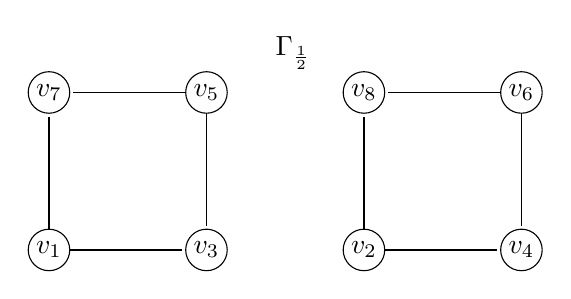
\begin{tikzpicture}[shorten >=1pt,auto,node distance=2cm,
thin,main node/.style = {circle,draw, inner sep = 0pt, minimum size = 15pt}]

\node[main node,fill=white] (1) {$v_1$};
\node[main node,fill=white] [right of = 1](2) {$v_3$};
\node[main node,fill=white] [above of = 1](3) {$v_7$};
\node[main node,fill=white] [above of =2](4) {$v_5$};
\node[main node,fill=white] [right of =2](5) {$v_2$};
\node[main node,fill=white] [right of = 5](6) {$v_4$};
\node[main node,fill=white] [above of = 5](7) {$v_8$};
\node[main node,fill=white] [above of =6](8) {$v_6$};
\node at (3.1,2.5) (9) {$\Gamma_{\frac{1}{2}}$};

\path[-]
(1) edge node {} (2)
edge node {} (3)
(4) edge node {} (3)
edge node {} (2)
(5) edge node {} (6)
edge node {} (7)
(8) edge node {} (7)
edge node {} (6);
\end{tikzpicture}\]
Alternatively, if we consider $U_2$, $\Gamma_{\frac{1}{\sqrt{2}}}$ is given below.
\[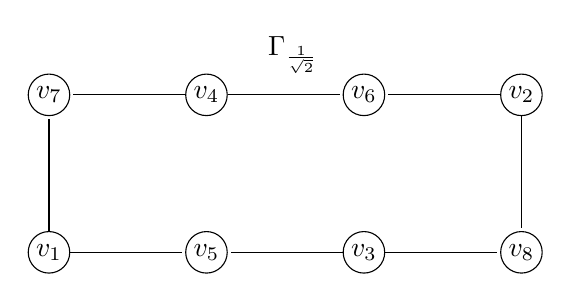
\begin{tikzpicture}[shorten >=1pt,auto,node distance=2cm,
	thin,main node/.style = {circle,draw, inner sep = 0pt, minimum size = 15pt}]
	
	\node[main node,fill=white] (1) {$v_1$};
	\node[main node,fill=white] [right of = 1](2) {$v_5$};
	\node[main node,fill=white] [above of = 1](3) {$v_7$};
	\node[main node,fill=white] [above of =2](4) {$v_4$};
	
	\node[main node,fill=white] [right of =2](5) {$v_3$};
	\node[main node,fill=white] [right of = 5](6) {$v_8$};
	\node[main node,fill=white] [above of = 5](7) {$v_6$};
	\node[main node,fill=white] [above of =6](8) {$v_2$};
	\node at (3.1,2.5) (9) {$\Gamma_{\frac{1}{\sqrt{2}}}$};
	
	\path[-]
	(1) edge node {} (2)
	edge node {} (3)
	(4) edge node {} (3)
	edge node {} (7)
	(5) edge node {} (6)
	edge node {} (2)
	(8) edge node {} (7)
	edge node {} (6);
\end{tikzpicture}\]
Thus $U_1$ and $U_2$ are non-isomorphic as their corresponding graphs are non-isomorphic double covers of $C_4$. We similarly define the five relations $R_0,\dots,R_4$ any $OPD_m(\gamma)$ via the inner products $1$, $\gamma$, $0$, $-\gamma$, and $-1$ respectively so that, for instance, $(x,y)\in R_2$ if and only if the corresponding vectors are orthogonal. These five relations satisfy all the requirements of an association scheme except for possibly the existence of intersection numbers. In the case of the first $OPD$, we find that even though both $(v_1,v_5)$ and $(v_1,v_6)$ are in $R_2$,
\[\left\vert\left\{v_x : (v_x,v_1),(v_5,v_x)\in R_{\gamma}\right\}\right\vert\neq\left\vert\left\{v_x : (v_x,v_1),(v_6,v_x)\in R_{\gamma}\right\}\right\vert.\]
On the other hand, the second $OPD$ has well-defined intersection numbers and we find that the columns of $U_2$, along with the relations $R_0,\dots,R_4$, give the association scheme $C_8$.
\end{example}
As one might expect, there are many graphs for which we cannot find an orthogonal projective double in the dimension given by the independence number. In other words, Proposition \ref{cocliquebnd} is often not tight. To see an example, consider the following proposition

\begin{prop}\label{completemulti}
	Let $\Gamma$ be a complete multipartite graph with $w$ parts of size $v$. Let $U$ be the matrix with columns corresponding to an $OPD_{\alpha(\Gamma)}(\gamma)$ of $\Gamma$. Then a subset of the columns of $U$ form a set of $w$ mutually unbiased bases in $\mathbb{R}^v$.
\end{prop}
\begin{proof}
	Follow the same proof as in Proposition \ref{cocliquebnd}, however only consider one line from each antipodal pair. Noting that non orthogonal vectors must have inner product $\pm\gamma$, the result is immediate.
\end{proof}
\begin{cor}\label{nonexist}
	Let $\Gamma = K_{2\times t}$ for $t\neq 0\mod 4$. There does not exist an $OPD_{\alpha(\Gamma)}(\gamma)$ of $\Gamma$.
\end{cor}
\begin{proof}
	If $K_{2\times t}$ had an orthogonal projective double, Proposition \ref{completemulti} would guarantee the existence of two mutually unbiased bases in $\mathbb{R}^t$. This is only possible when $t$ is a multiple of $4$.
\end{proof}

\section{Schemes induced by projective doubles}
Example \ref{doublecoverc4} provides an orthogonal projective double which naturally gives an association scheme on the vectors. In this section, we consider which graphs produce such an association scheme and some properties of the association scheme which arise. First, let $L = \left\{\ell_i\right\}$ be an orthogonal projective double of some graph $\Gamma$ and let $G$ be the Gram matrix of $L$; that is, the matrix whose entry in row $i$ and column $j$ is $\left<\ell_i,\ell_j\right>$. We denote by $\left<G\right>_\circ$ the vector space of matrices generated by $G$ using entrywise products. Note that the adjacency matrices of each graph $\Gamma_{\theta}$ for $\theta\in\left\{\pm 1,\pm \gamma,0\right\}$ are all contained in $\left<G\right>_{\circ}$. Thus $\left<G\right>_\circ$ is a Bose-Mesner algebra if and only if it is closed under standard matrix multiplication. If this occurs, we say $L$ induces the corresponding 4-class association scheme. Thus, from example \ref{doublecoverc4}, the association scheme $C_8$ is induced by the columns of $U_2$. We similarly define $\left<A\right>_*$ for any matrix $A$ and note that this algebra is a Bose-Mesner algebra if and only if it is closed under Schur products.

A \emph{strongly regular graph}\index{strongly regular graph} (see \cite{Brouwer1989}) with parameters $(v,k,\lambda,\mu)$ is a $k$-regular graph with $v$ points where every pair of adjacent vertices have exactly $\lambda$ neighbors in common while distinct non-adjacent vertices have $\mu$ neighbors in common. Using the terminology of association schemes, a strongly regular graph is a 2-class association scheme with parameters $k = p^0_{11}$, $\lambda = p^1_{11}$ and $\mu = p^2_{11}$.

\projsrg
%\begin{prop}\label{projnec}
%	A projective double of a simple graph $\Gamma$ induces an association scheme only if $\Gamma$ is strongly regular.
%\end{prop}
\begin{proof}
	We will prove our result by showing that $\overline{\Gamma}$, the complement of $\Gamma$, is strongly regular. Define $v = \vert V\Gamma\vert$ and let $L = \left\{\ell_1,\dots,\ell_{2v}\right\}$ be our $OPD$ with the projective mapping $\phi:L\rightarrow V\Gamma$. First let $R_0,\dots,R_4$ be the relations of the association scheme induced by $L$ where $R_2$ is given by orthogonality, $R_0$ is the identity relation, and the remaining relations are given by the inner products $\gamma,-\gamma,$ and $-1$ respectively. By definition of our mapping, $\phi(\ell)=\phi(\ell^\prime)$ for $\ell\neq \ell^\prime$ if and only if $\ell=-\ell^\prime$. Thus for distinct vertices $u,w\in V\Gamma$, $u\not\sim w$ if and only if $\phi^{-1}(w)\subset \phi^{-1}(u)^\perp$. Then the number of vertices not adjacent to $u$ is half the number of vectors orthogonal to either vector in $\phi^{-1}(u)$; this value is $\frac{1}{2}p^0_{22}$. Similarly, assuming $u\not\sim w$, the number of vertices adjacent to neither $u$ nor $w$ must be half the number of vectors orthogonal to any pair of vectors, one from $\phi^{-1}(v)$ and the other from $\phi^{-1}(w)$; that is, $\frac{1}{2}p^2_{22}$. Similarly, assume $v\sim w$ and we find the number of vertices adjacent to neither $v$ nor $w$ must be $\frac{1}{2}p^1_{22} = \frac{1}{2}p^3_{22}$. Thus $\overline{\Gamma}$ is strongly regular with parameters $(\vert\Gamma\vert,\frac{1}{2}p^0_{22},\frac{1}{2}p^{2}_{22},\frac{1}{2}p^1_{22})$.
\end{proof}

This proposition tells us that we must only consider strongly regular graphs if we wish to find orthogonal projective doubles which induce association schemes. Note that the converse of Proposition \ref{projnec} is certainly not true; the first projective double of Example \ref{doublecoverc4} does not result in an association scheme even though $C_4$ is strongly regular. Thus we will look for further necessary or sufficient conditions for a $OPD$ to induce an association scheme. Before we continue, we review a few details of strongly regular graphs which will be useful for us.

Let $\Gamma$ be a strongly regular graph with parameters $(v,k,\lambda,\mu)$. Let $R_1$ be the relation given by adjacency in $\Gamma$ and define parameters $r,s,f,g$ so that the spectrum of $\Gamma$ is $k^1,r^f,s^g$. Using the first and second orthogonality relations (Lemma \ref{orthorels}) we find the first and second eigenmatrices of the association scheme are:
\begin{equation}\label{PQsrg}P = \left[\begin{array}{ccr}
1 & k & v-k-1\\
1 & r & -(r+1)\\
1 & s & -(s+1)
\end{array}\right],\qquad Q = \left[\begin{array}{ccc}
1 & f & g\\
1 & \frac{fr}{k} & \frac{gs}{k}\\
1 & \frac{f(1+r)}{k+1-v} & \frac{g(1+s)}{k+1-v}
\end{array}\right].\end{equation}
The following lemma from \cite{Brouwer1989}, shows us that the parameters $k,r,$ and $s$ are sufficient to define all other parameters as long as $k+rs\neq 0$. In the case of $k+rs=0$, $\Gamma$ is a union of cliques and $v$ is not uniquely determined by the spectrum---we will ignore this case in much of our discussion.
\begin{lem}\cite[Theorem.~1.3.1.(iii,vi)]{Brouwer1989}\label{srgparams} Whenever $k+rs>0$, the parameters of a strongly regular graph may be expressed in terms of $r$, $s$, and $k$ with $g = v-f-1$:
	\[\mu = k+rs, \qquad v = \frac{(k-r)(k-s)}{\mu},\qquad \lambda = \mu+r+s,\qquad f = \frac{(s+1)k(k-s)}{\mu(s+r)}.\]
\end{lem}
The association scheme structure allows us to improve on the naive upper bound given in Corollary \ref{regnaive} by using the techniques discussed in Section \ref{equilines}.
\begin{thm}
	Let $\Gamma$ be a strongly regular graph with spectrum $k^1,r^f,s^g$ $(r>s)$. There exists an $OPD_{f+1}(\gamma)$ of $\Gamma$.
\end{thm}
\begin{proof}
	Let $A_0$, $A_1$, and $A_2$, be the adjacency matrices of the identity graph, $\Gamma$, and $\overline{\Gamma}$ respectively. From equation \eqref{PQsrg}, $E_1 = \frac{1}{v}\left(fA_0 + \frac{fr}{k}A_1 + \frac{f(1+r)}{k+1-v}A_2\right)$. Then 
	\[G = \frac{(1+r)}{v-k-1}E_0 + \frac{1}{f}E_1 = \left(\frac{v+r-k}{v(v-k-1)}\right)A_0 +\left(\frac{k+r(v-1)}{v(v-k-1)}\right)A_1\]
	is a $v\times v$ positive semi-definite matrix with rank $f+1$ with the off diagonal entries we seek. We may then find a matrix $U$ such that $\left(\frac{v(v-k-1)}{v+r-k}\right)G = U^TU$, that is, the columns of $U$ are unit vectors in $\mathbb{R}^{f+1}$ such that $u_i\perp u_j$ if and only if the corresponding points in $X$ are related by $R_2$. Then $L = \left\{\pm u_1,\dots,\pm u_v\right\}$ is an $OPD_{f+1}\left(\frac{k+r(v-1)}{v+r-k}\right)$ of $\Gamma$ where $u_i$ is the $i^\text{th}$ column of $U$.
\end{proof}
Note that this construction does not induce a 4-class association scheme. We see this by noting that all off diagonal entries in $G$ must be positive. Thus we may split our $OPD$ into two sets $L^+$ and $L^-$ where $L^+$ contains all the columns of $U$ and $L^-$ contains their negatives. Then for vectors $u\perp v$, the number of vectors $w$ such that $\left<v,w\right> = \left<u,w\right>=\gamma$ could be either $0$ (if $v\in L^+$ and $u\in L^-$) or $\lambda$ (if $v,w\in L^+$). Thus this value is not solely dependent on the inner product $\left<u,v\right>$ and $p^2_{11}$ is not well defined. While this does not solve our question of which $OPD$'s induce association schemes, it does provide us with a better upper bound on the dimension needed for strongly regular graphs. For example, this gives an $OPD$ of the Petersen graph in dimension $5$ while Corollary \ref{regnaive} produces one in dimension $9$. Now consider the following theorem of Delsarte.

\begin{thm}\cite{Delsarte1973} \label{delsarte}
	Let $\Gamma$ be a strongly regular graph with $v$ vertices, valency $k$, and smallest eigenvalue $s$. If $C$ is a coclique of $\Gamma$, then
	\[\vert C\vert\leq v\left(1-\frac{k}{s}\right)^{-1}, \]
	with equality if and only if every vertex $\gamma\notin C$ has the same number of neighbors (namely $-s$) in $C$.\qed
\end{thm}
We will refer to a \emph{Delsarte coclique}\index{Delsarte coclique} as a coclique for which this bound is tight. This theorem, along with Proposition \ref{cocliquebnd}, gives a lower bound on the dimension of any $OPD$ in terms of the spectrum whenever $\Gamma$ contains a Delsarte coclique. Further, we may use the final line of Theorem \ref{delsarte} to learn more information about any $OPD$ achieving this bound.
\cocliquealpha
%\begin{cor}\label{snegsquare}
%	Let $\Gamma$ be a nonempty strongly regular graph with $v$ vertices, valency $k$ and smallest eigenvalue $s$ which contains a Delsarte coclique $C$. Then any projective double in $\mathbb{R}^{\vert C\vert}$ has inner product $\gamma=\sqrt{-s}$. Further, either $\Gamma$ is complete bipartite or $\gamma^{-1}\in \mathbb{Z}$.
%\end{cor}
\begin{proof}
	Let $L$ be the $OPD_{\vert C\vert}(\gamma)$ of $\Gamma$. Further, let $\ell_1,\dots,\ell_{\vert C\vert}$ be vectors in $L$ such that the set $\left\{\phi(\ell_1),\dots,\phi(\ell_{\vert C\vert})\right\}$ is a Delsarte coclique. Then $\left\{\ell_1,\dots,\ell_{\vert C\vert}\right\}$ forms an orthonormal basis for $\mathbb{R}^{\vert C\vert} = \text{span}(L)$. Let $a\in L$ be given with $\phi(a)\notin C$. By Theorem \ref{delsarte}, $\phi(a)$ must be adjacent to exactly $-s$ points in $C$ and thus, reordering the vectors and replacing $\ell_i$ with $-\ell_i$ as needed, we may assume $\left<a,\ell_i\right> = \gamma$ for $1\leq i\leq -s$. Therefore $a = \sum_{i=1}^{-s} \gamma\ell_i$ implying that $-s\gamma^2 = 1$ and thus $s = -\gamma^{-2}$. Now, as long as $\Gamma$ is not complete bipartite, there must be another vector $b\in L$ for which $\phi(b)\notin C$ and $\phi(b) \sim\phi(a)$; assume $\left<b,a\right> = \gamma$ taking $-b$ if needed. We again find that $\phi(b)$ is adjacent to exactly $-s$ vertices in $C$; let $h$ be the number of vertices adjacent to both $a$ and $b$. Without loss of generality $b =  \sum_{i=1}^{h} \beta_i\ell_i + \sum_{i=-s+1}^{-2s-h}\gamma\ell_i$ where $\beta_i = \pm\gamma$. Thus $\left<a,b\right> = (p-q)\gamma^2$ where $p$ is the number of vectors in $\left\{\ell_1,\dots,\ell_h\right\}$ with $\left<b,\ell_i\right> = \left<a,\ell_i\right>$ and $q = h-p$. However, since $a$ and $b$ have inner product $\gamma$, this implies $\gamma^{-1} = p-q$.
\end{proof}
While this theorem only provides information about $OPD$'s of strongly regular graphs with Delsarte cocliques, there are many common examples which contain these cocliques for which we may apply our theorem. For instance, consider the following result.
\begin{cor}
	There do not exist $OPD$'s for either the Petersen graph in $\mathbb{R}^4$ or the 9-Paley graph in $\mathbb{R}^3$. 
\end{cor}
\begin{proof}
	Recall that the Petersen graph has 10 vertices, valency 3, and smallest eigenvalue $-2$. Thus a Delsarte coclique has size $\bigslant{10}{\left(1+\frac{3}{2}\right)} = 4$; we may verify quickly that such a coclique exists. Thus Corollary \ref{snegsquare} tells us a projective double of the Petersen graph in $\mathbb{R}^4$ would require that $\sqrt{-s}$ is an integer, which is false. Similarly the 9-Paley graph has 9 vertices, valency 4, and smallest eigenvalue $-2$. Using the same reasoning, noting that here a Delsarte coclique has size 3, we have our result.
\end{proof}


\begin{thm}\label{dimtoassociation}
	Let $\Gamma$ be a strongly regular graph with $v$ vertices, valency $k$, and smallest eigenvalue $s$ with $k+rs>0$. Let $G$ be the Gram matrix of an $OPD_m(\gamma)$ of $\Gamma$ with $m = v\left(1+k\gamma^2\right)^{-1}$. Then $\left<G\right>_\circ$ is the Bose-Mesner algebra of a 4-class association scheme.
\end{thm}
\begin{proof}
	We begin by ordering the vectors in our orthogonal projective double so that $\ell_1,\dots,\ell_v$ are representatives from distinct lines and $\ell_{i+v} = -\ell_{i}$ for $1\leq i\leq v$. Likewise we order the vertices of $\Gamma$ so that $\ell_i$ and $\ell_{v+i}$ are mapped to vertex $i$. Let $G$ be the Gram matrix of our $OPD_m(\gamma)$ of $\Gamma$ with rows and columns ordered in this fashion; that is $G_{ij} = \left<\ell_i,\ell_j\right>$ for $1\leq i,j\leq 2v$. This ordering implies there exists a matrix $\tilde{G}$ such that
	\[G =\def\arraystretch{1.4}\left[\begin{array}{c:c}
	\tilde{G} & -\tilde{G}\\\hdashline[2pt/2pt]
	-\tilde{G} & \tilde{G}\\[2pt]
	\end{array}\right].\]
	Now let $\tilde{A}_1$ and $\tilde{A}_2$ be the adjacency matrices of $\Gamma$ and $\overline{\Gamma}$ respectively. Let $\tilde{E}_0$, $\tilde{E}_1$, and $\tilde{E}_2$ be the minimal idempotents corresponding to the eigenvalues $k$, $r$, and $s$ respectively; that is, $\tilde{A}_1\tilde{E}_0 = k\tilde{E}_0$, $\tilde{A}_1\tilde{E}_1 = r\tilde{E}_1$, and $\tilde{A}_1\tilde{E}_2 = s\tilde{E}_2$. For both the adjacency matrices and the minimal idempotents, assume the rows and columns are ordered via the ordering defined above. Recall that the second eigenmatrix of this association scheme is
	\[\tilde{Q} = \left[\begin{array}{ccc}
	1 & f & g\\
	1 & \frac{fr}{k} & \frac{gs}{k}\\
	1 & \frac{f(r+1)}{k+1-v} & \frac{g(s+1)}{k+1-v}
	\end{array}\right].\]
	
	We now define 5 matrices $E_0,\dots,E_4$, which we will show are orthogonal idempotents. For the first two, define $E_0 = \frac{1}{2v}J$ and $E_1 = \frac{m}{2v}G$. We then define $E_2$ and $E_4$ entrywise based on the values of $G$
	\[2v\left[E_2\right]_{ij} = \begin{cases}
	f & \text{ if }G_{ij} = \pm1\\
	\frac{fr}{k} & \text{ if }G_{ij} = \pm\gamma\\
	\frac{f(r+1)}{k+1-v} & \text{ if }G_{ij} = 0\\
	\end{cases}\qquad 2v\left[E_4\right]_{ij} = \begin{cases}
	g & \text{ if }G_{ij} = \pm1\\
	\frac{gs}{k} & \text{ if }G_{ij} = \pm\gamma\\
	\frac{g(s+1)}{k+1-v} & \text{ if }G_{ij} = 0\\
	\end{cases}.\]
	Our final matrix will be $E_3 = I-E_0-E_1-E_2-E_4$.	First note that our definitions for $E_0$, $E_2$, and $E_4$ imply
	\[E_0 =\frac{1}{2}\def\arraystretch{1.4}\left[\begin{array}{c:c}
	\tilde{E}_0 & \tilde{E}_0\\\hdashline[2pt/2pt]
	\tilde{E}_0 & \tilde{E}_0\\[2pt]
	\end{array}\right],\qquad E_2 = \frac{1}{2}\def\arraystretch{1.4}\left[\begin{array}{c:c}
	\tilde{E}_1 & \tilde{E}_1\\\hdashline[2pt/2pt]
	\tilde{E}_1 & \tilde{E}_1\\[2pt]
	\end{array}\right],\qquad E_4 = \frac{1}{2}\def\arraystretch{1.4}\left[\begin{array}{c:c}
	\tilde{E}_2 & \tilde{E}_2\\\hdashline[2pt/2pt]
	\tilde{E}_2 & \tilde{E}_2\\[2pt]
	\end{array}\right].\]
	It follows that the set $\left\{E_0,E_2,E_4\right\}$ is a set of orthogonal idempotents. In order to show $E_1$ is a fourth idempotent, recall that $G = \frac{2v}{m}E_1$ is a Gram matrix and we find $GJ = \left(1+k\gamma-k\gamma-1\right)J = 0$; thus $G$ is the Gram matrix of a $1$-design. We may then use the second degree Gegenbauer polynomial (see equation \eqref{gegdef}) to show that
	\[\sum_{j}Q_2^m\left(G_{ij}\right) = \frac{m\left(2+2k\gamma^2\right)-2v}{m-1} = \frac{2m\left(1+k\gamma^2\right)-2v}{(m-1)}=0\]
	for any choice of $1\leq i\leq 2v$. Thus Theorem 5.3 of \cite{Delsarte1977} tells us $G$ is the Gram matrix of a $2$-design and must have eigenvalues $\frac{2v}{m}$ and $0$. This implies the symmetric matrix $E_1$ has eigenvalues $1$ and $0$; therefore $E_1$ is idempotent. Additionally, the block structure of the matrices $E_0$, $E_1$, $E_2$, and $E_4$ imply that $E_1E_0=E_1E_2=E_1E_4 = 0$ telling us that the set $\left\{E_0,E_1,E_2,E_4\right\}$ is a set of orthogonal idempotents. We now consider our fifth matrix and note that, using the fact that the other four matrices are orthogonal idempotents, we find
	\[E_3^2 = \left(I-E_0-E_1-E_2-E_4\right)^2 = I-E_0-E_1-E_2-E_4\]
	and $E_3E_i = 0$ for $i\neq 3$. We therefore have that the matrix algebra spanned by $\left\{E_0,E_1,E_2,E_3,E_4\right\}$ is closed under matrix multiplication and contains both the identity matrix and the all ones matrix. In order to show this algebra is a Bose-Mesner algebra, we must also show it is closed under entrywise products. We do this by listing the corresponding Krein parameters and verifying element-wise that $E_i\circ E_j = \frac{1}{2v}\sum_{k=0}^4q^k_{ij}E_k$. In the matrices that follow, we refer to the parameter definitions in Theorem \ref{srgparams} for the strongly regular graph parameters.
	\[L_0^* =  \left[ \begin {array}{ccccc} 1&0&0&0&0\\ \noalign{\medskip}0&1&0&0&0
	\\ \noalign{\medskip}0&0&1&0&0\\ \noalign{\medskip}0&0&0&1&0
	\\ \noalign{\medskip}0&0&0&0&1\end {array} \right],\qquad L_1^* = \left[\begin{array}{ccccc}
	0 & m & 0 & 0 & 0\\
	1 & 0 & \frac{f(1+r\gamma^2)}{1+k\gamma^2} & 0 & \frac{g(1+s\gamma^2)}{1+k\gamma^2}\\
	0 & \frac{m(1+r\gamma^2)}{1+k\gamma^2} & 0 & \frac{\gamma^2(k-r)m}{1+k\gamma^2} & 0\\
	0 & 0 & \frac{f(k-r)}{k(1+k\gamma^2)} & 0 & \frac{g(k-s)}{k(1+k\gamma^2)}\\
	0 & \frac{m(1+s\gamma^2)}{1+k\gamma^2} & 0 & \frac{\gamma^2(k-s)m}{1+k\gamma^2}
	\end{array}\right],\]
	\[L_2^* =   \left[ \begin {array}{ccccc} 0&0&f&0&0\\
	\noalign{\medskip}0&{\frac {\left( {\gamma}^{2}r+1 \right)f }{  \left( {\gamma}^{2}k+1 \right) }}&0&{\frac {
			\left( k-r \right) {\gamma}^
			{2}f}{ \left( {\gamma}^{2}k+1
			\right) }}&0\\
	\noalign{\medskip}1&0&f-1+{\frac { \left( k-r
			\right)gs}{ \left( r-s \right)k }}&0&{-\frac { \left( k-r
			\right)gs}{ \left( r-s \right)k }}\\
	\noalign{\medskip}0&{\frac { f\left( k-r \right) }{ k\left( {\gamma}^{2}k+1 \right) }}&0&{\frac { \left( {\gamma}^{2}{k}^{2}+r \right)f }{
			k  \left( {\gamma}^{2}k+1
			\right) }}&0\\ \noalign{\medskip}0&0&{-\frac {\left( k-r \right) sf}{ \left( r-s \right)k }}&0&{\frac { \left( k-s \right) r f }{ \left( r-s \right) k }}
	\end {array} \right],\]
	 \[L_3^* = \left[ \begin {array}{ccccc} 0&0&0&m{\gamma}^{2}k&0\\
	 \noalign{\medskip}0&0&{\frac {f{\gamma}^{2} \left( k-r
			\right) }{{\gamma}^{2}k+1}}&0&{\frac {g{\gamma}^{2} \left( k-s
			\right) }{{\gamma}^{2}k+1}}\\
		\noalign{\medskip}0&{\frac {m{\gamma}^{
				2} \left( k-r \right) }{ {\gamma}^{2}k+1 }}&0&{
		\frac {m{\gamma}^{2} \left( {\gamma}^{2}{k}^{2}+r \right) }{ {
				\gamma}^{2}k+1}}&0\\ \noalign{\medskip}1&0&{\frac {f
			\left( {\gamma}^{2}{k}^{2}+r \right) }{k \left( {\gamma}^{2}k+1
			\right) }}&0&{\frac {g \left( {\gamma}^{2}{k}^{2}+s \right) }{k
			\left( {\gamma}^{2}k+1 \right) }}\\ \noalign{\medskip}0&{\frac {m{
				\gamma}^{2} \left( k-s \right) }{  {\gamma}^{2}k+1}
	}&0&{\frac {{\gamma}^{2} \left( {\gamma}^{2}{k}^{2}+s \right) }{
			{\gamma}^{2}k+1}}&0\end {array} \right],\]
	\[ L_4^* = \left[ \begin {array}{ccccc} 0&0&0&0&g
	\\ \noalign{\medskip}0&{\frac {g \left( {\gamma}^{2}s+1 \right) }{\left( {\gamma}^{2}k+1 \right) }}&0&{\frac {
			\left( k-s \right) {\gamma}^{2}g }{\left( {\gamma}^{
				2}k+1 \right) }}&0\\
	\noalign{\medskip}0&0&-{\frac {\left( k-r \right)gs}{ \left( r-s \right)k}}&0&{\frac { \left( k-s \right) r g }{ \left( r-s \right) k }}
	\\ \noalign{\medskip}0&{\frac { \left( k-s \right) g }{k
			  \left( {\gamma}^{2}k+1 \right) }}&0&{\frac { g \left( {\gamma}^{2}{k}^{2}+s \right) }{
			k\left( {\gamma}^{2}k+1
			\right) }}&0\\
	\noalign{\medskip}1&0&{\frac { \left( k-s \right)rf }{ \left( r-s \right) k  }
	}&0&g-1-\frac{(k-s)rf}{(r-s)k}\end {array} \right].\]
Therefore the algebra generated by $\left<E_0,\dots,E_4\right>$ is the Bose-Mesner algebra of a 4-class association scheme. Since $G = \frac{2v}{m}E_1$, it is clear that $\left<G\right>_\circ\subset\text{span}\left\{E_0,\dots,E_4\right\}$. For the other direction we use the adjacency matrices of this Bose-Mesner algebra. Define $c_i$ for $0\leq i\leq 4$ via $G\circ A_i = c_iA_i$ and we have
\[A_i = \prod_{j\neq i}\left(\frac{G-c_jJ}{c_i-c_j}\right)\]
where the product is taken entrywise.
\end{proof}
\begin{cor}
	\label{delcocliquetoqbip}
	Let $\Gamma$ be a strongly regular graph with $v$ vertices, valency $k$, and smallest eigenvalue $s$ with $k+rs>0$ which contains a Delsarte coclique. Let $G$ be the Gram matrix of an $OPD_m(\gamma)$ of $\Gamma$ with $m = v\left(1-\frac{k}{s}\right)^{-1}$. Then $\left<G\right>_\circ$ is the Bose-Mesner algebra of a 4-class $Q$-bipartite association scheme.
\end{cor}
\begin{proof}
	Corollary \ref{cocliquebnd} tells us that $\gamma = \frac{1}{\sqrt{s}}$ and therefore $m = v\left(1+k\gamma^2\right)$. Then Theorem \ref{dimtoassociation} gives that $\left<G\right>_\circ$ is the Bose-Mesner algebra of a 4-class association scheme. The bipartite property follows as $(1+s\gamma^2) = 0$, implying $L_1^*$ is tridiagonal.
\end{proof}

Theorem \ref{dimtoassociation} tells us that $OPD$'s of strongly regular graphs induce association schemes whenever the dimension is tight with respect to Proposition \ref{cocliquebnd}. It turns out this is also a sufficient condition as long as the dimension is not too far away from optimal; that is, $m<v$. Consider the following theorem.
\begin{thm}\label{genqbip}
	Let $\Gamma$ be a strongly regular graph with $v$ vertices, valency $k$, and smallest eigenvalue $s$. Let $L$ be an $OPD_m(\gamma)$ of $\Gamma$ with $m<v$. $L$ induces an association scheme only if $m = v\left(1+k\gamma^2\right)^{-1}$. Further, either $\text{rank}\left(G\circ G\right)=v$ or the induced scheme is $Q$-bipartite and $s=-\gamma^{-2}$.
\end{thm}
\begin{proof}
	We prove this by building the $Q$ matrix of the resultant scheme. First let $\BMA = \left<G\right>_\circ$ and $\BMB = \left<A_\Gamma\right>_*$ where $A_\Gamma$ is the adjacency matrix of $\Gamma$. Since $G$ has five distinct values, $\BMA$ must be a 4-class association scheme with basis matrices $A_0,A_1,A_2,A_3,$ and $A_4$ corresponding to the values $1,\gamma,0,-\gamma,$ and $-1$. By definition of an $OPD$, we find that $R_0\cup R_4$ gives a system of imprimitivity where $\BMB$ is the quotient algebra of $\BMA$. Since $\cI = \left\{0,4\right\}$, the matrix $A_0+A_4$ must be one basis matrix; the other two matrices are $A_1+A_3$ and $A_2$. Further, there exist three basis idempotents of $\BMA$, call them $E_0$, $E_2$, and $E_4$, which span the same subalgebra as $A_0+A_4$, $A_1+A_3$, and $A_2$. By Lemma \ref{repeatedcols}, we must have $\tilde{Q}_{\tilde{k}j} = Q_{kj}$ for $j\in\left\{0,2,4\right\}$ and $0\leq k\leq 4$ where $\tilde{Q}$ is the second eigenmatrix of the strongly regular graph. Equation \eqref{PQsrg} tells us this matrix is
	\[\tilde{Q} = \left[\begin{array}{ccc}
	1 & f & g\\
	1 & \frac{fr}{k} & \frac{gs}{k}\\
	1 & \frac{f(1+r)}{k+1-v} & \frac{g(1+s)}{k+1-v}
	\end{array}\right]\]
	and thus the second eigenmatrix of $\BMA$ must be ($*$ denotes an unknown value)
	\[Q = \left[\begin{array}{crcrc}
	1 & * & f & * & g\\
	1 & * & \frac{fr}{k}  & * & \frac{gs}{k}\\
	1 & * & \frac{f(r+1)}{k+1-v}  & *& \frac{g(1+s)}{k+1-v}\\
	1 & * & \frac{fr}{k} & * & \frac{gs}{k}\\
	1 & * & f & * & g\\
	\end{array}\right].\]
	Let $n_1$ and $n_3$ be the remaining two multiplicities corresponding to $E_1$ and $E_3$ respectively. Since $1+f+g=v$ and $\vert X\vert = 2v$, we must have $n_1+n_3 = v$. Now, by construction, $G = A_0 + \gamma A_1 -\gamma A_3 -A_4$ and therefore any diagonal entry of $GE_2$ is given by
	\[\left[GE_2\right]_{ii} = \frac{1}{\vert X\vert}\left(f+k\left(\frac{fr}{k}\right)\gamma - k\left(\frac{fr}{k}\right)\gamma -f\right) = 0.\]
	Similarly, the diagonal entries of both $GE_4$ and $GE_0$ are also $0$. This tells us that $\text{tr}(GE_0) = \text{tr}(GE_2) = \text{tr}(GE_4)=0$. Since $G$ is assumed to be contained within this commutative algebra, we find $GE_i = E_iG$ for each idempotent $E_i$ and therefore the matrices $GE_4$, $GE_2$, and $GE_0$ are all symmetric. This forces $GE_0=GE_2=GE_4=0$ since each product must be positive semi-definite. Thus there exists constants $c_1$ and $c_3$ such that $G = c_1E_1+c_3E_3$. Since $m<v$, only one of these constants may be non-zero; without loss of generality assume $c_3 =0$. This gives $n_1 = m$ and $G = \frac{\vert X\vert}{m}E_1$. Therefore $G^2 = \frac{\vert X\vert^2}{m^2}E_1 = \frac{\vert X\vert}{m}G$ and we must have
	\[\left[G^2\right]_{11} = 2\left(1+k\gamma^2\right) = \frac{\vert X\vert}{m},\]
	implying $m = v\left(1+k\gamma^2\right)^{-1}$.
	
	Now we may return to our $Q$ matrix and fill in the entries of the first column. Further, the orthogonality relations (Lemma \ref{orthorels}) tell us that $\sum_{j}Q_{ij} = \delta_{0j}\vert X\vert$. Using the same fact for $\tilde{Q}$, we may find the final column as well. 
	\[Q = \left[\begin{array}{crccc}
	1 & m & f & v-m & g\\
	1 & m\gamma & \frac{fr}{k}  & -m\gamma & \frac{gs}{k}\\
	1 & 0 & \frac{f(r+1)}{k+1-v}  & 0& \frac{g(1+s)}{k+1-v}\\
	1 & -m\gamma & \frac{fr}{k} & m\gamma & \frac{gs}{k}\\
	1 & -m & f & m-v & g\\
	\end{array}\right]\]
	Since we now have the entire $Q$ matrix, we may use Lemma $\ref{kitchensink}$ $(xiii^\prime)$ to find the Krein parameters of our scheme. In particular we find that $q^3_{11} = q^4_{12} = 0$ as well as
	\[\begin{aligned}q^2_{11} &= \frac{1}{2v f}\sum_{h=0}^d\left(k_hQ_{h1}Q_{h1}Q_{h2}\right) = \frac{m^2\left(1+\gamma^2r\right)}{v},\\
	q^3_{12} &= \frac{1}{2v (v-m)}\sum_{h=0}^d\left(k_hQ_{h1}Q_{h2}Q_{h3}\right) = \frac{mf\left(v-m(1+\gamma^2r)\right)}{v(v-m)},\\
	q^4_{13} &= \frac{1}{2v g}\sum_{h=0}^d\left(k_hQ_{h1}Q_{h3}Q_{h4}\right) = \frac{m\left(v-m(1+\gamma^2s)\right)}{v}.\\	
	\end{aligned}\]
	Noting that $v- m(1+\gamma^2r)>v-m(1+\gamma^2k) = 0$ as long as $r\neq k$ ($\Gamma$ is not a union of cliques) we have all three Krein parameters nonzero. Thus $\BMA$ is $Q$-polynomial if and only if $q^{4}_{11}=0$. Calculating this similarly, we find
	\[q^4_{11} = \frac{1}{2v g}\sum_{h=0}^d\left(k_hQ_{h1}Q_{h1}Q_{h4}\right) = \frac{m^2g\left(1+\gamma^2s\right)}{v}.\]
	We therefore find $q^4_{11}=0$ if and only if $s = -\gamma^{-2}$. Finally, since $q^0_{11},q^2_{11}>0$, we have $\text{rank}(G\circ G) = 1+f+g=v$ if $q^4_{11}>0$ and $\text{rank}(G\circ G) = 1+f<v$ otherwise.
\end{proof}
\dimiffassoc
\begin{proof}
	The result follows immediately from Theorems \ref{genqbip} and \ref{dimtoassociation}.
\end{proof}

From these results we are very close to the statement ``The association scheme induced by a $OPD_m(\gamma)$ is $Q$-bipartite if and only if $\gamma = \frac{1}{\sqrt{-s}}$", however this statement is ultimately false. Consider the Gram matrix of any $OPD_m(\frac{1}{\sqrt{-s}})$ with $m = v\left(1-\frac{k}{s}\right)^{-1}$, following the proof of Theorem \ref{genqbip} we find that $\left<G\right>_\circ$ generates a $Q$-bipartite association scheme with $E_1 = \frac{m}{2v}G$. However, in this case, $\frac{2v}{v-m}E_3$ is the Gram matrix of an $OPD_{v-m}\left(\frac{m}{(v-m)\sqrt{-s}}\right)$. Further, since $E_3$ has five distinct entries just as $E_1$, we find that $\left<G\right>_\circ = \left<\frac{2v}{v-m}E_3\right>_\circ$ and thus we have an $OPD$ which generates a $Q$-bipartite association scheme without $\gamma = \frac{1}{\sqrt{-s}}$. It is the belief of this author that this is the only obstruction to our statement. We note that this requires $v-m>m$ else it would violate Corollary \ref{cocliquebnd}. Therefore we can avoid this issue by requiring $m<\frac{v}{2}$, guaranteeing our Gram matrix is the first idempotent in the $Q$-polynomial ordering.
\begin{conj}
	Let $\Gamma$ be a strongly regular graph with $v$ vertices, valency $k$, and smallest eigenvalue $s$. An $OPD_m(\gamma)$ of $\Gamma$ in dimension $m<\frac{v}{2}$ induces an association scheme if and only if either $m = v\left(1-\frac{k}{s}\right)^{-1}$. Further, the association scheme induced is $Q$-bipartite.
\end{conj}
\section{4-class $Q$-bipartite association schemes}
Theorem \ref{genqbip} and Corollary \ref{cocliquebnd} indicated that nearly any orthogonal projective double of a strongly regular graph which induces an association scheme must induce a 4-class $Q$-bipartite scheme. As we saw in Corollary \ref{nonexist}, many complete multipartite graphs will not have any orthogonal projective doubles in the dimension required to induce an association scheme. In general, the existence of an $OPD$ for $K_{n,m}$ which induces an association scheme is equivalent to the existence of a set of mutually unbiased bases in the same dimension. These are exactly the 4-class $Q$-bipartite schemes which are also $Q$-antipodal (\cite{LeCompte2010}). We will ignore these cases and assume that the underlying strongly regular graph is not complete multipartite. For the remaining 4-class $Q$-bipartite schemes, we examine the eigenmatrices and find that the parameters of such a scheme are completely determined by the spectrum of the quotient strongly regular graph. We will begin by showing that the parameters of any such scheme are determined completely by the spectrum of the quotient SRG. We then recast Theorem \ref{cometricbnds} in terms of these three parameters and derive explicit bounds for this case which are required for the parameter set to be realizable. Let $(X,\mathcal{R})$ be a 4-class $Q$-bipartite association scheme, not also $Q$-antipodal, with $Q$-polynomial ordering $E_0,E_1,\dots,E_4$ and natural ordering $A_0,A_1,\dots A_4$. We know from Theorem \ref{suzukiimprim} that the quotient of $(X,\mathcal{R})$ has exactly two non-trivial relations and thus must be strongly regular. Let $(v,k,\lambda,\mu)$ be the parameters of the quotient strongly regular graph corresponding to $A_1+A_3$. Let $k>r>s$ be the eigenvalues of this SRG with corresponding multiplicities $1$, $f$, and $g$. Since $(X,\mathcal{R})$ is not $Q$-antipodal, we must have $k>r$ and $s>-k$. The $Q$ matrix of this SRG will be
\[\tilde{Q} = \left[\begin{array}{ccc}
1 & f & g\\
1 & \frac{fr}{k} & \frac{gs}{k}\\
1 & \frac{f(1+r)}{k+1-v} & \frac{g(1+s)}{k+1-v}
\end{array}\right].\]
We may use this information to build the first and second eigenmatrices of our $4$-class $Q$-bipartite scheme as follows.
\begin{thm}
	\label{Pmat}
	Let $(X,\mathcal{R})$ be a 4-class $Q$-bipartite association scheme with relations ordered naturally. Let the quotient SRG have $v$ vertices and spectrum $k^1,r^f,s^g$ with $k>r>s$. Then the first and second eigenmatrices are as follows:
	\[P = \left[\begin{array}{crcrr}
	1 & k & 2(v-1-k) & k & 1\\
	1 & \frac{k}{n} & 0 & -\frac{k}{n} & -1\\
	1 & r& -2(1+r) & r & 1\\
	1 & -n & 0 & n & -1\\
	1 & s & -2(s+1) & s & 1\\
	\end{array}\right]\qquad Q = \left[\begin{array}{crcrc}
	1 & m & f & \frac{mk}{n^2} & g\\
	1 & \frac{m}{n} & \frac{fr}{k}  & -\frac{m}{n} & \frac{gs}{k}\\
	1 & 0 & \frac{f(r+1)}{k+1-v}  & 0& \frac{g(1+s)}{k+1-v}\\
	1 & -\frac{m}{n} & \frac{fr}{k} & \frac{m}{n} & \frac{gs}{k}\\
	1 & -m & f & \frac{mk}{n^2} & g\\
	\end{array}\right]\]
	where $s = -n^2$.
\end{thm}
\begin{proof}
	We begin by building all of $Q$ and then employ the use of our orthogonality properties. Note that column 0 of $Q$ comes by definition. From Theorem [\cite{Brouwer2003},\cite{Martin2007}], $Q_{1,1} = -Q_{3,1}\neq 0 = Q_{2,1}$, so we define $n = \frac{m}{Q_{1,1}} = -\frac{m}{Q_{3,1}}$ and column 1 is given. Each entry in columns 2 and 4 follow from Lemma \ref{repeatedcols}. Finally column 3 may be found using the first orthogonality condition (specifically that $\displaystyle{\sum_j Q_{ij} = \vert X\vert\delta_{i0}}$). From here we have that 
	\[Q = \left[\begin{array}{crccc}
	1 & m & f & v-m & g\\
	1 & \frac{m}{n} & \frac{fr}{k}  & -\frac{m}{n} & \frac{gs}{k}\\
	1 & 0 & \frac{f(r+1)}{k+1-v}  & 0& \frac{g(1+s)}{k+1-v}\\
	1 & -\frac{m}{n} & \frac{fr}{k} & \frac{m}{n} & \frac{gs}{k}\\
	1 & -m & f & m-v & g\\
	\end{array}\right],\]
	matching our theorem in all but two places.	Since we have ordered the relations using the natural ordering, the valencies of our relations are given by $[1,k,2(v-1-k),k,1]$. This allows us to derive an expression for $q_{01}^1$ using \cite[Theorem.~2.3.2.]{Brouwer1989} which gives
	\[q_{ij}^k = \frac{1}{\vert X\vert m_k}\sum_{l=0}^d\left(v_lQ_{li}Q_{lj}Q_{lk}\right)\]
	where $m_k$ and $v_l$ are the multiplicities and valencies of the $k^\text{th}$ and $l^\text{th}$ relations respectively. We find that $q_{01}^1 = \frac{1}{2vm}\left(2m^2+\frac{2km^2}{n^2}\right)$, however we know from Theorem \ref{kitchensink} that $q_{01}^1=1$, resulting in $\frac{km}{n^2} = v-m$. This completes our proof for the second eigenmatrix and we may use the second orthogonality condition to find $P$ noting that the first row of $P$ is the valencies of our relations. Thus
	\[P = \left[\begin{array}{crcrr}
	1 & k & 2(v-1-k) & k & 1\\
	1 & \frac{k}{n} & 0 & -\frac{k}{n} & -1\\
	1 & r& -2(1+r) & r & 1\\
	1 & -n & 0 & n & -1\\
	1 & s & -2(s+1) & s & 1\\
	\end{array}\right].\]
	We again use our equation for Krein parameters one more time to find $q_{11}^4 = \frac{mg(n^2+s)}{n^2v}$. Since $q_{11}^4=0$ due to our cometric property, we have that $s = -n^2$.
\end{proof}
\begin{cor}
	The parameters of a 4-class $Q$-bipartite scheme are uniquely determined by the eigenvalues of the quotient SRG.
\end{cor}
\begin{proof}
	Our first eigenmatrix only requires $v,k,r,s,$ and $n$. However since $n>0$ due to the natural ordering of relations, $n = \sqrt{-s}$. The remaining parameter is given in Lemma \ref{srgparams}. 
\end{proof}
Before moving to examine the effect of Sch\"{o}nberg's theorem on 4-class $Q$-bipartite schemes, we mention a few parameter bounds arising from the feasibility conditions FC1-FC3 and show how they restrict the space of feasible parameters.
\begin{thm}
	\label{bounds}
	Suppose we have a feasible parameter set for a $4$-class association scheme which is $Q$-bipartite but not $Q$-antipodal. Let $k=P_{01}$, $r=P_{21}$, and $s=P_{41}$ where $P$ is the first eigenmatrix using the natural ordering. The following must hold with $n:=\sqrt{-s}$ and $\mu=k+rs$:
	\begin{enumerate}[label=(\roman*)]
		\item $\mu\geq n(r+n)$,
		\item $n\vert \mu$ and $n\vert k$,
		\item $r\geq \frac{2k}{3n^2}-\frac{n^2}{3}$,
		\item $kn^2(n^2-1)\geq \mu(n^2+r)$
	\end{enumerate}
	Further, $n$ is an integer greater than 1.
\end{thm}
\begin{proof}
	First note that $k$, $r$, and $s$ are the eigenvalues of a strongly regular graph and thus integral (we assume here that the SRG is not a conference graph). For $(i)$ and $(ii)$, note that	$p_{13}^1 = \frac{(n-1)(\mu-n(r+n))}{2n}$. FC2 tells us that this must be a non-negative integer, and therefore we must either have $-s = n = 1$ or $\mu-n(r+n)\geq0$. As $s=-1$ implies our SRG is a union of cliques (and thus $(X,\mathcal{R})$ is $Q$-antipodal), we may ignore this case and $(i)$ follows. Since $\gcd(n,n-1)=1$, we have that $n\vert (\mu-n(r+n))$ forcing $n\vert \mu$ and since $k=\mu+rn^2$, $(ii)$ follows. Next, $(iii)$ follows from the absolute bound $1+f \leq \frac{m(m+1)}{2}$ giving us $n^4+3n^2r-2k\geq 0$. Using another absolute bound, $(iv)$ follows from $\frac{v}{m}\leq f$. Finally, since $n = \sqrt{-s}$, if $n$ is not an integer, then columns one and three of $Q$ must be irrational. However Galois conjugation is an automorphism of our Bose-Mesner algebra and thus $E_0$, $E_3$, $E_2$, $E_1$, $E_4$ must be a second $Q$ polynomial ordering in this case, implying $q_{3,3}^4=0$. Using our $P$ and $Q$ matrices, we find that $q_{3,3}^4 = \frac{(k-r)(k+s)}{\mu}$. This means that whenever $n$ is irrational, either $r=k$ or $s = -k$, both of which imply $(X,\mathcal{R})$ is $Q$-antipodal.
\end{proof}

\begin{cor}
	\label{kbnds}
	Suppose we have a feasible parameter set for a $4$-class association scheme which is $Q$-bipartite but not $Q$-antipodal. Let $k=P_{01}$, $r=P_{21}$, and $s=P_{41}$ where $P$ is the first eigenmatrix using the natural ordering. Then
	\[\frac{k}{n^2}-1\leq \frac{(n+1)}{2}\left((n+1)(n^3-n-1)+\sqrt{(n-1)(n^7+3n^6+2n^5-4n^4-9n^3-3n^2+3n-1)}\right).\]
\end{cor}
\begin{proof}
	Using Theorem \ref{bounds}$(i)$ and $(iv)$, we have that $n(r+n)\leq \mu\leq \frac{kn^2(n^2-1)}{n^2+r}$. Using $\mu = k-rn^2$, these two inequalities give us
	\[\frac{k-n^4+\sqrt{n^8-2n^4k(2n^2+3)+k^2}}{2n^2}\leq r\leq \frac{k-n^2}{n(n+1)}.\]
	This implies that 
	\[k^2-n^2(n^5+2n^4-3n^2-3n+1)k+n^5(n^2+n-1)\leq0.\]
	When $k=1$ and $n>1$, the left hand side will be negative. Therefore this requires that $k$ is less than the positive root of this quadratic, giving us our bound.
\end{proof}
We now examine the bounds arising from Corollary \ref{Qbipbnds} as applied to our 4-class $Q$-bipartite association scheme. We begin by noting that $\theta_{31}\geq 0$ becomes Theorem \ref{bounds} $(i)$ when we use the parameters $k$, $r$, and $n$, thus making it equivalent to an absolute bound in this context. Next, we find that plugging in our parameters gives $\theta_{42}\geq 0$ and $\theta_{53}\geq 0$ if and only if $k\geq \frac{-rn^2}{n^2-2}$ and $k\geq -\frac{(3n^2-7)rn^2}{n^4-3n^2+6}$ respectively. Both of these bounds are vacuous since the right hand side will be negative for any choice of $n>1$. Finally one may show that $\theta_{31}\geq 0$ and $\theta_{60}\geq 0$ together imply $\theta_{51}\geq 0$ in the specific case of a 4-class $Q$-bipartite scheme. Therefore the only new restriction, not implied by FC1-FC3 is $\theta_{60}\geq 0$, resulting in the following theorem.
\fourclasssixzero
\begin{comment}\begin{thm}\label{thm60}
Suppose we have a feasible parameter set for a $4$-class association scheme which is $Q$-bipartite but not $Q$-antipodal. Let $k=P_{01}$, $r=P_{21}$, and $s=P_{41}$ where $P$ is the first eigenmatrix using the natural ordering. Then the scheme is realizable only if
\[15n^4(2n^2-3)r^2 + (n^6-45kn^2+76k)n^2r+k(16k+n^6)(n^2-2)\geq 0.\]
\end{thm}
\end{comment}
\begin{proof}
	Apply the parameters $k,r,$ and $s$ to Theorem \ref{Qbipbnds} $(v)$.
\end{proof}
We may pair this Theorem with Theorem \ref{bounds} to get the following corollary.
\begin{cor}\label{newkbnds}
	Suppose we have a feasible parameter set for a $4$-class association scheme which is $Q$-bipartite but not $Q$-antipodal. Let $k=P_{01}$, $r=P_{21}$, and $s=P_{41}$ where $P$ is the first eigenmatrix using the natural ordering. The following table gives an upper bound on the largest eigenvalue $k$ based on the smallest $s$ for $-4\leq s\leq 121$:
	\[\begin{tabular}{c|c|c|c|c|c|c|c|c|c|c}
	$n$ & 2 & 3 & 4 & 5 & 6 & 7 & 8 & 9 & 10 & 11\\\hline
	$k\leq$  & 56 & 891 & 5504 & 22297 & 85128 & 282828 & 867787 & 2609805 & 8468529 & 40926495\\
	\end{tabular}\]
\end{cor}
\begin{proof}
	Let $r_1\geq r_2$ be the two roots of $15n^4(2n^2-3)r^2 + (n^6-45kn^2+76k)n^2r+k(16k+n^6)(n^2-2)$. Then Theorem \ref{thm60} tells us that either $r\geq r_1$ or $r\leq r_2$. Pairing this with Theorem $\ref{bounds}$ we find that $r\geq r_1$ and $\mu\geq n(r+n)$ together restrict $k$ via
	\[\begin{aligned}	\frac{k}{n^3(n^2-1)}&\leq \frac{n^7+2n^6-3n^4-17n^3+45n^2+14n-76}{-2(n^4-13n^3+15n^2+12n-32)(n^2-1)}\\
	&\qquad+\frac{\sqrt{n^{10}+4n^9+6n^8+2n^7-35n^6+22n^5+145n^4-72n^2+32n+16}}{-2(n^4-13n^3+15n^2+12n-32)}.\end{aligned}\]
	Secondly, $r\leq r_2$ with $r\geq\frac{2k}{3n^2}-\frac{n^2}{3}$ implies that $k\leq \frac{3n^6-5n^4}{2}$. Taking the maximum of these two bounds for each $2\leq n\leq 11$ results in the values given in the table. In each case apart from $n=11$, this is a reduction from the bound given in Theorem \ref{kbnds}
\end{proof}
We conclude this chapter by noting the impact of Theorem \ref{thm60} on the feasible parameter space of 4-class $Q$-bipartite association schemes. In the table below we list the number of feasible schemes for a given $n>0$ when only considering conditions FC1, FC2, and FC3. We also list the number of feasible schemes when we include Theorem \ref{thm60} as a feasibility condition.
\[\begin{tabular}{c|c|c}\label{feasible4class}
$n$ & \# of feasible parameter sets & \# of feasible parameter sets satisfying Theorem \ref{thm60}\\\hline
2 & 6 & 5\\
3 & 60 & 44\\
4 & 223 & 140\\
5 & 473 & 334\\
6 & 1015& 701\\
7 & 1256& 952\\
8 & 2256& 1659\\
\end{tabular}\]
The following figures display the original feasibility conditions and the new bound due to $\theta_{60}\geq 0$. We display the graphs for $n=7$, noting that similar graphs may be generated for any $n>1$.
\begin{figure}[h]
	\begin{subfigure}[h]{0.5\textwidth}
		\includegraphics[scale=.5]{bounds7py.png}
	\end{subfigure}
	\begin{subfigure}[h]{0.5\textwidth}
		\includegraphics[scale=.5]{geg7.png}
	\end{subfigure}
	\caption[4-class $Q$-bipartite bounds]{These figures pertain to the case $n = 7$. On the left we have two absolute bounds and a bound due to the non-negativity of an intersection number. In green, we have plotted every parameter set which is feasible under FC1-FC3. On the right, we have replaced the bounds with the bound $\theta_{60}\geq 0$. Any parameter set contained within the parabola is not realizable.}
\end{figure}